\section{Antiderivadas}

 Si $F'(x)=f(x),$ diremos que $F$ es una antiderivada de $f.$

 \begin{problema}
  \label{soc:exmp:22.1}
  $x^{3}$ es una antiderivada de $3x^{2},$ porque...  
  $$
  D_{x}\left( x^{3} \right)=3x^{2}
  $$  
  Pero $x^{3}+5$ es también una antiderivada de $3x^{2},$ porque...  
  $$
  D_{x}\left( x^{3} +5 \right)=3x^{2}
  $$
 \end{problema}



 En general, si $F(x)$ es una antiderivada de $f(x),$ entonces $F(x)+C, \, C\in \R$ es también una antiderivada.
 

 Más aun, si $F(x)$ y $G(x)$ son antiderivadas de $f(x),$ entonces existe $C\in \R$ tal que
 $$
 F(x)=G(x)+C.
 $$
 

 Diremos que $C$ es una \emph{constante de integraci\'on.}



 $\int f(x)dx$ denotara cualquier antiderivada de $f(x)$ más una constante de integraci\'on.
 

 Diremos que $f(x)$ es el integrando, mientras que $\int f(x)dx$ es llamada \emph{integral indefinidad.}



 \begin{problema}
 \label{soc:exmp:22.2}
  \begin{enumerate}
   \item $$\int xdx= \dfrac{1}{2}x^{2}+C$$
   
   \item $$\int -\sin(x)dx=  \cos(x)+C$$
  \end{enumerate}

 \end{problema}




 \begin{prop}[Reglas para antiderivadas]
  \begin{enumerate}
  \label{antiderivatives}
   \item $\int 0 dx=C$
   
   \item $\int 1 dx=x+C$
   
   \item $\int adx=ax+C$
   
   \item $\int x^{r}dx=\dfrac{x^{r+1}}{r+1}+C, \, r\neq-1$
   
   \item $\int af(x)dx=aF(x)+C$
   
   \item $\int \left( f(x)+g(x) \right)dx=\int f(x)dx+\int g(x)dx$
   
   \item $\int \left( f(x)-g(x) \right)dx=\int f(x)dx-\int g(x)dx$
  \end{enumerate}

 \end{prop}




 \begin{problema}
  \label{soc:exmp:22.3}
  \begin{enumerate}
   \item $\int \sqrt[3]{x}dx=$
   
   \item $\int \frac{1}{x^{2}}dx=$
   
   \item $\int 7x^{3}dx=$
   
   \item $\int \left( x^{2}+4 \right)dx=$
   
   \item $\int \left( 3x^{6}-4x \right)dx=$
   
  \end{enumerate}

 \end{problema}




  Con las reglas (3)-(7), podemos calcular la antiderivada de cualquier polinomio.
 \begin{problema}
  \label{soc:exmp:22.4}
  $$\int \left( 6x^{8}-\frac{2}{3}x^{5}+7x^{4}+\sqrt{3} \right)dx=$$
 \end{problema}



\subsection{Integración por sustitución}


 \begin{prop}[Integración por sustitución]
 \label{regla:8}
 $$\int \left( g(x) \right)^{r}g'(x)dx=
 \dfrac{1}{r+1}\left( g(x) \right)^{r+1}+C
 $$ para $r\neq -1.$
 \end{prop}




 \begin{problema}
  \label{soc:exmp:22.5}
  $$
  \int \left( \dfrac{1}{3}x^{3}+7 \right)^{5}x^{2}dx=
  $$
 \end{problema}




 \begin{problema}
  \label{soc:exmp:22.6}
  $$
  \int \left( x^{2}+1 \right)^{2/3}xdx=
  $$
 \end{problema}




 \begin{prop}[Regla 9, método de sustituci\'on]
  \label{regla:9}
  $$
  \int f\left( g(x) \right)g'(x)dx=\int f(u)du
  $$
  donde $u=g(x), du=g'(x)dx.$
 \end{prop}

 Véase el ejericicio resuelto \ref{soc:solved:22.21}



 \begin{problema}
  \label{soc:exmp:22.7.a}
  Encuentre $$\int x \sin(x^{2})dx=$$
 \end{problema}




 \begin{problema}
  \label{soc:exmp:22.7.b}
  Encuentre $$\int  \sin(x/2)dx=$$
 \end{problema}



 
  \begin{figure}
 \centering
 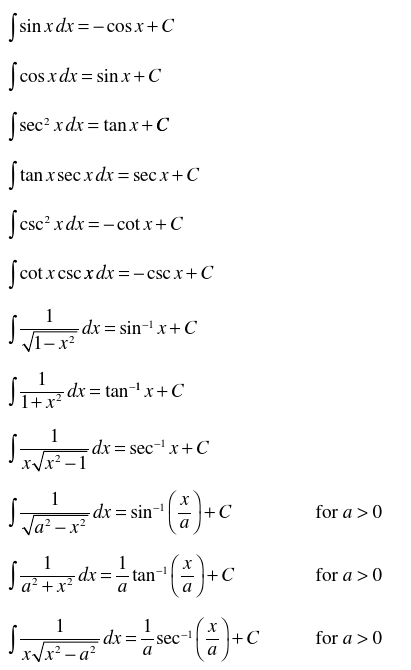
\includegraphics[height=.8\textheight]{./calculo/antiderivadas.png}
 % antiderivadas.png: 0x0 pixel, 300dpi, 0.00x0.00 cm, bb=
 \caption{Antiderivadas comunes}
 \label{fig:antiderivadas}
\end{figure}

 


 \subsection{Ejemplos Resueltos}


 
  \begin{problema}[F\'ormula de integración por sustitución \eqref{regla:8}]
   \begin{enumerate}
    \item $\int \left( s^{3}+2 \right)^{2}(3s^{2})ds=$ 
    \item $\int \left( x^{3}+2 \right)^{1/2}x^{2}dx=$ 
    \item $\int \dfrac{8x^{2}}{\left( x^{3}+2 \right)^{3}}dx=$
    
    \item $\int\dfrac{x^{2}dx}{\sqrt[4]{x^{3}+2}}dx=$
    
    \item $\int 3x\sqrt{1-2x^{2}}dx=$
    
    \item $\int \sqrt[3]{1-x^{2}}xdx=$
    
    \item $\int \sin^{2}(x)\cos(x)dx=$
   \end{enumerate}


  \end{problema}

 


 \begin{problema}
  \begin{enumerate}
   \item $\int \dfrac{\cos(\sqrt{x})}{\sqrt{x}}dx=$
   
   \item $\int x\sec^{2}(4x^{2}-5)dx=$
   
   \item $\int x^{2}\sqrt{x+1} dx=$
  \end{enumerate}

 \end{problema}




 
  \begin{problema}
  \label{soc:solved:22.19}
   Una piedra se lanza hacia arriba desde el suelo, con una velocidad inicial de $64ft/s.$
   \begin{enumerate}
    \item ¿Cuándo alcanzará su altura máxima?
    \item ¿Cuál será su altura máxima?
    \item ¿Cuándo tocará el suelo?
    \item ¿Cuál será su velocidad al tocar el suelo?
   \end{enumerate}

  \end{problema}

 



 \begin{problema}
 \label{soc:solved:22.20}
  Encuentre la ecuaci\'on de una curva en el plano $xy$ que pasa por el punto $(0,1)$ y cuya pendiente es igual a la altura en cada punto $(x,y).$
 \end{problema}




 \begin{problema}
  \label{soc:solved:22.21}
  Justifique el método de sustituci\'on \eqref{regla:9}.
 \end{problema}



%\subsection{Evaluaci\'on continua}
%
%

%\begin{problema}[Antiderivadas] En los siguientes Ejemplos, puede utilizar cualquier regla para antiderivadas.
%\begin{multicols}{2}
% \begin{enumerate}

%
% \end{enumerate}
%\end{multicols}
%\end{problema}
%
%
%
% \frametitle{Bibliografía}
% Las notas de estas secci\'on se basaron en el capítulo 22 \texttt{``Antiderivatives''} de nuestro libro de texto \texttt{``Ayres, F. and Mendelson, E.;\textbf{``Calculus''}; Schaum's Outlines, McGraw Hill; 5th Edition.''}
%
